\section{活動編輯}

\begin{frame}{活動編輯}
\begin{itemize}
\item 上火車之後忘了停錶\pause
\item 想獨立出畫圖的那段活動(比如把騎去泰北高中以及從泰北高中騎回宿舍的部份從神掌的活動中獨立出來)\pause
\item 想獨立出比賽的那段活動(比如開賽前$10$秒就會先按錶,但是那$10$秒影響了 Strava 上看到的成績)\pause
\item 計時失敗\pause
\item 想把畫圖騎錯路的地方刪掉\pause
\item 活動分成了兩段紀錄,想合併成一個活動(比如騎到助航站之後很興奮就先上傳活動了,回去之後想把去程與回程的合併在一起)
\end{itemize}
\end{frame}

\begin{frame}{Strava 內建功能(網頁版)}
\begin{multicols}{2}
\begin{itemize}
\only<1>{
\item 點三個點$\to$Crop/Split
\item Crop:裁切
\item Split:分割
\newpage
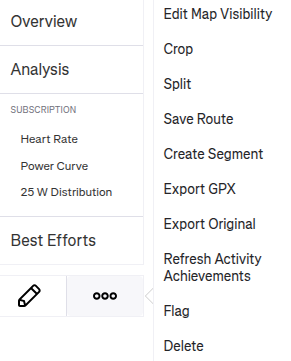
\includegraphics[height=6cm]{cropSplit.png}
}\only<2->{
\pause
\item 裁切:去頭去尾\\
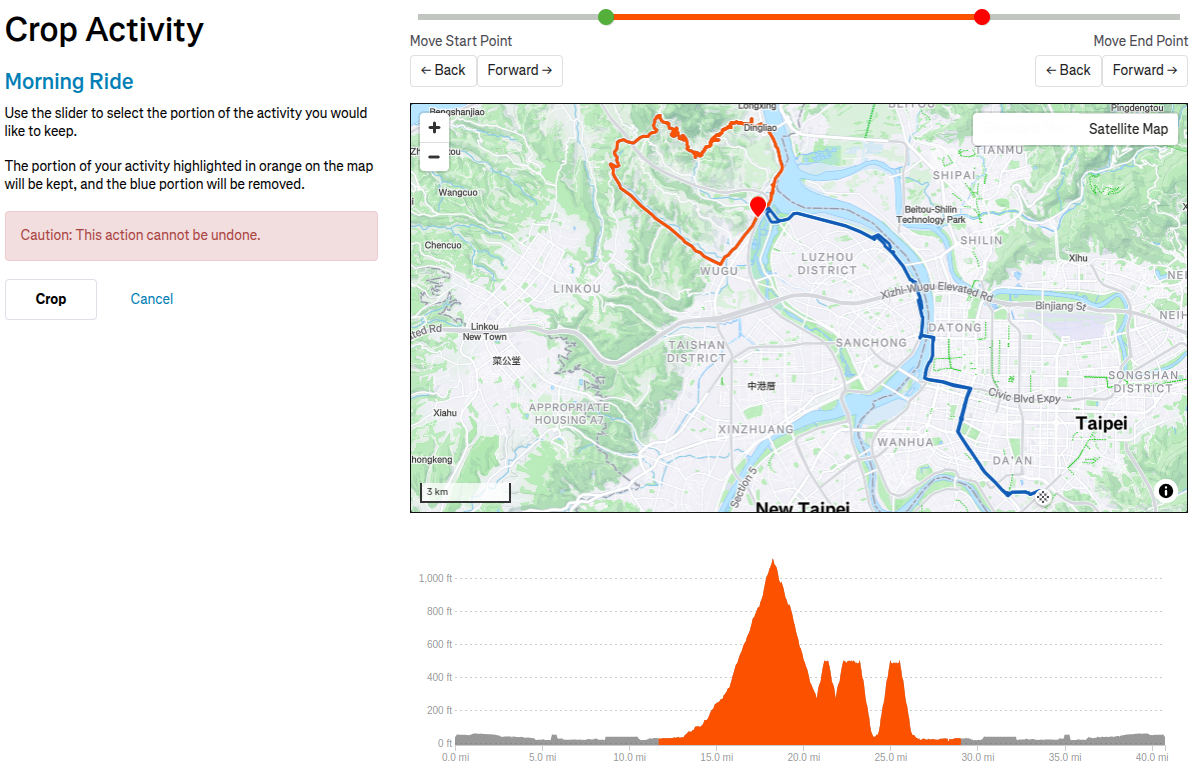
\includegraphics[width=7cm]{crop.png}\pause
\newpage
\item 分割成$2$或$3$個活動\\
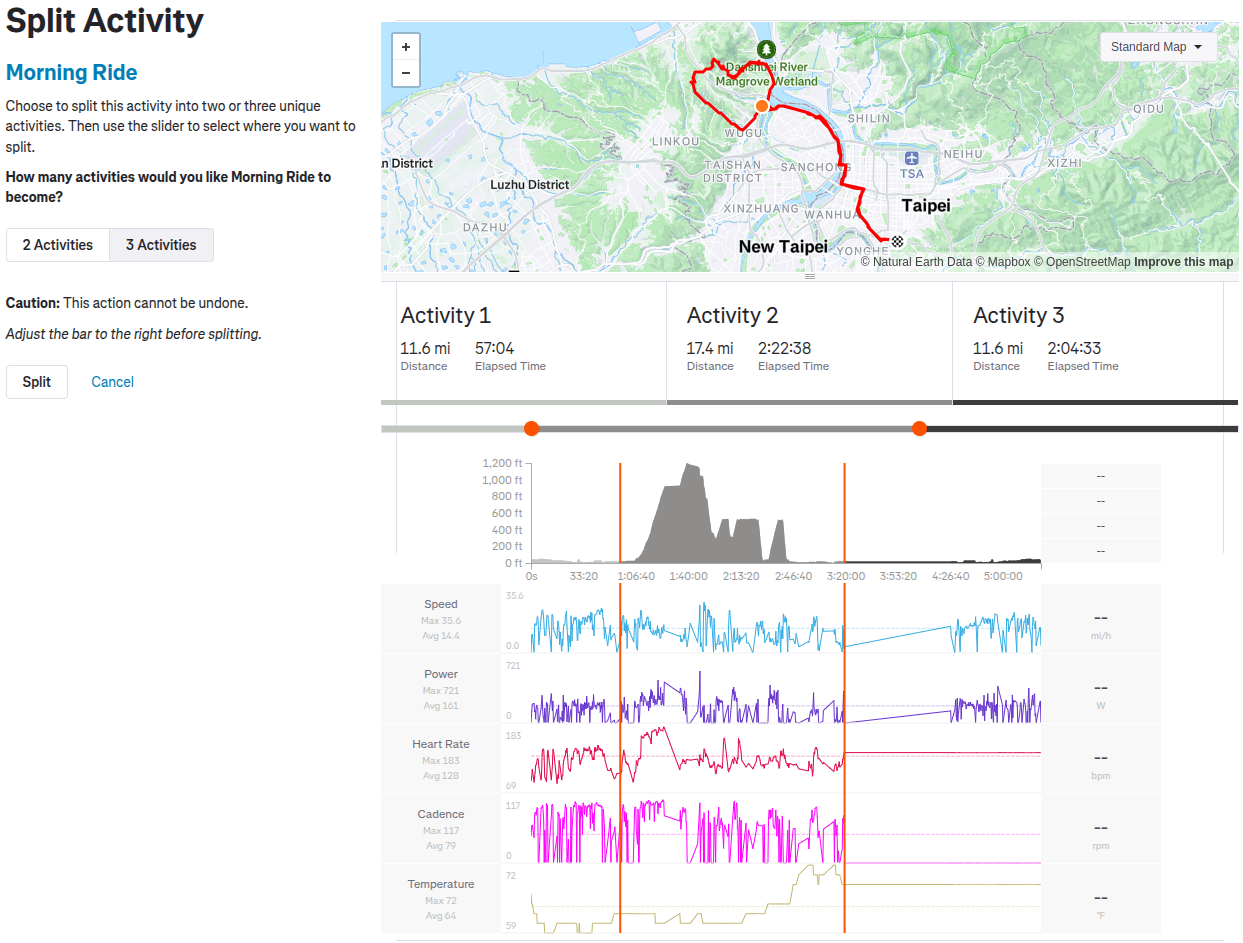
\includegraphics[width=7cm]{split.png}
}
\end{itemize}
\end{multicols}
\end{frame}

\begin{frame}[fragile]{合併活動(網頁版)}
\begin{multicols}{2}
\begin{itemize}
\item 點三個點$\to$Export GPX/Export Original\\
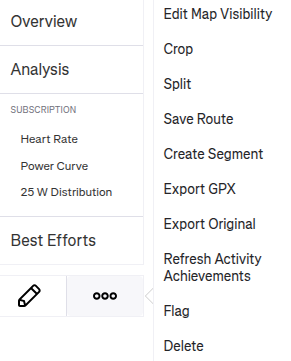
\includegraphics[height=5cm]{cropSplit.png}\pause
\item .fit:使用\href{https://www.fitfiletools.com/#/top}{這個網站}\pause
\item .gpx, .tcx, .csv:使用\href{https://gotoes.org/strava/}{這個網站}\pause
\item 常見問題:功率/心率資料遺失(未知原因)
\end{itemize}
\end{multicols}
\end{frame}

\begin{frame}{GPX 檔}
\begin{itemize}
\only<1-5>{
\item Strava 用來儲存一個活動的檔案格式,點選 Export GPX 可獲得一個活動的 .gpx 檔\pause
\item 自己的活動有經緯度、海拔、時間、功率、溫度、心率、踏頻,總之所有車錶有紀錄的東西\pause
\item 別人的活動只有經緯度、海拔\pause
\item 與 .xml 有相近的格式,可以使用 .xml 相關的 parser 來處理(例如 Python 的 \href{https://docs.python.org/3/library/xml.etree.elementtree.html}{xml.etree.ElementTree} ),需注意 namespace 的處理\pause
\item Meta data (左)與單個紀錄點(右):\\
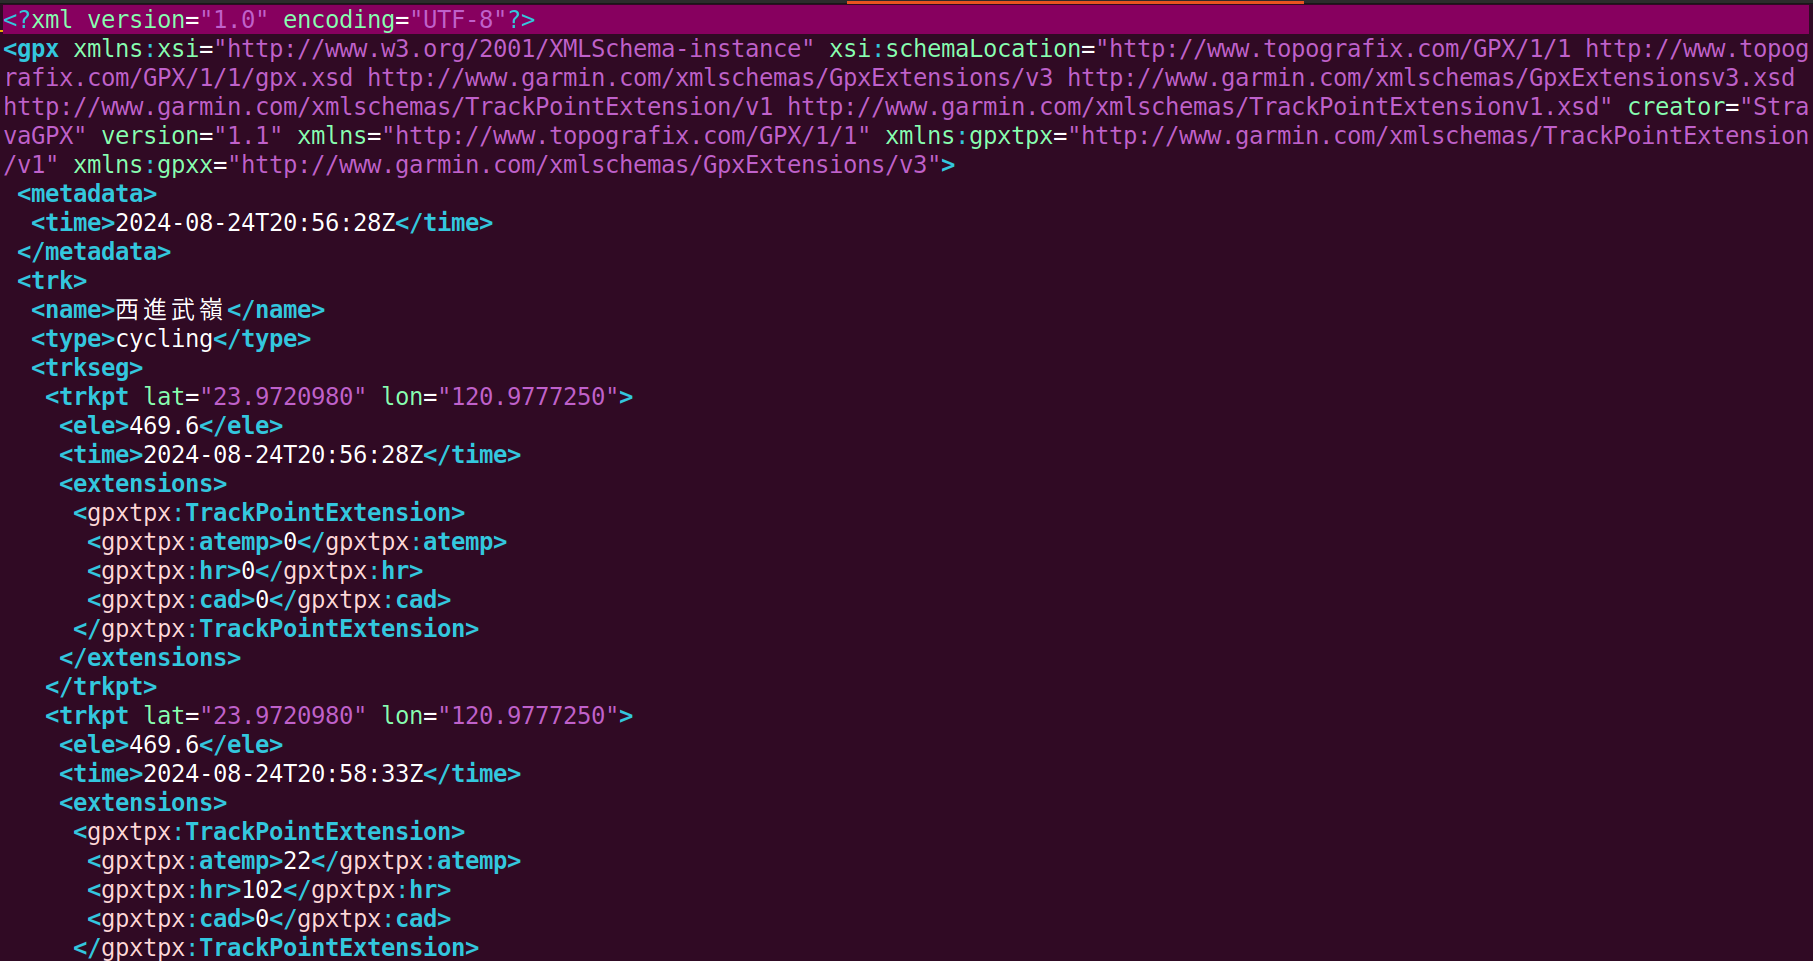
\includegraphics[width=7cm]{gpx1.png}
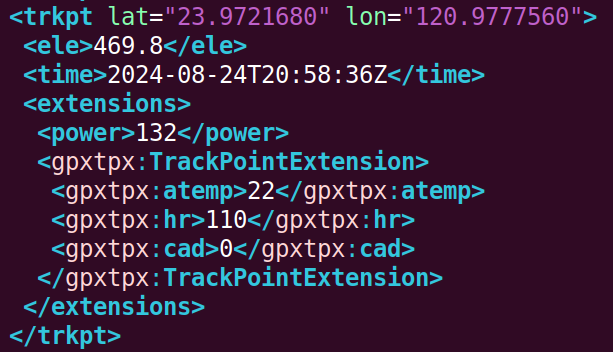
\includegraphics[width=7cm]{gpx2.png}
}\only<6->{
\begin{multicols}{2}
\pause\pause\pause\pause\pause
\item 車錶通常是 .fit 格式,上傳 Strava 會自動轉成 .gpx\pause
\item Q: 為什麼要用不同的格式?\pause
\item A: 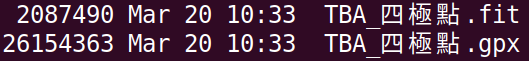
\includegraphics[width=7cm]{gpxFitCompare.png}\\\pause
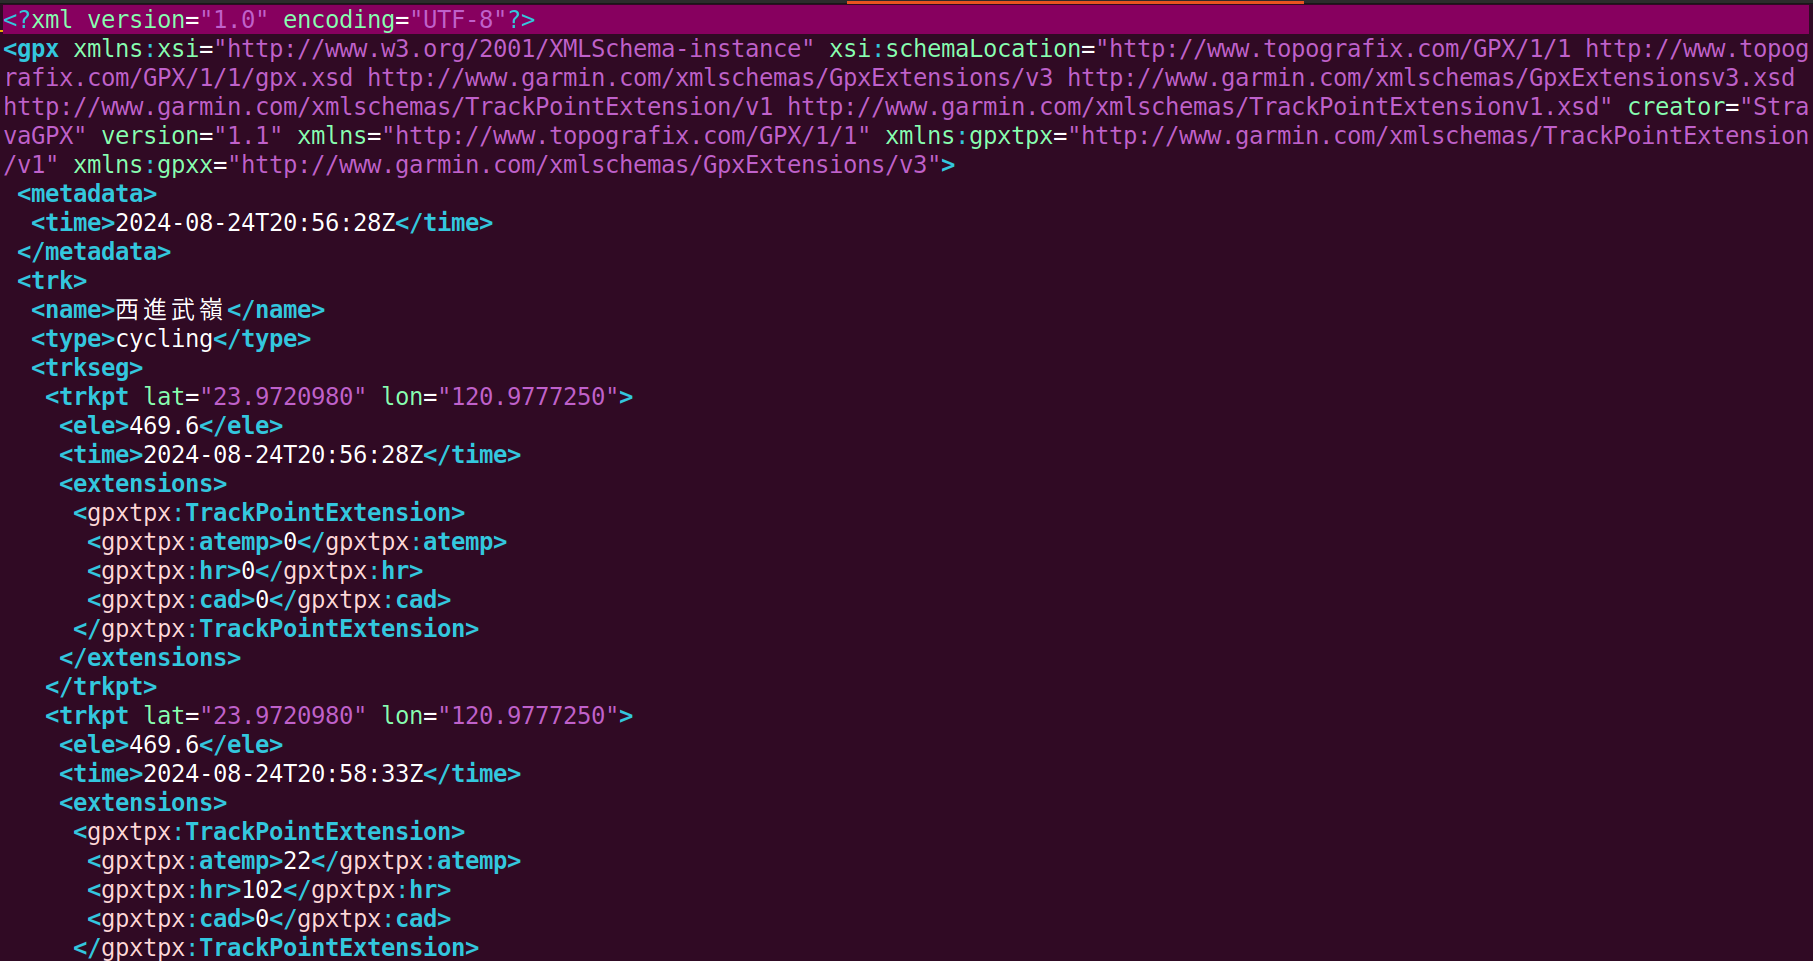
\includegraphics[width=7cm]{gpx1.png}
\newpage
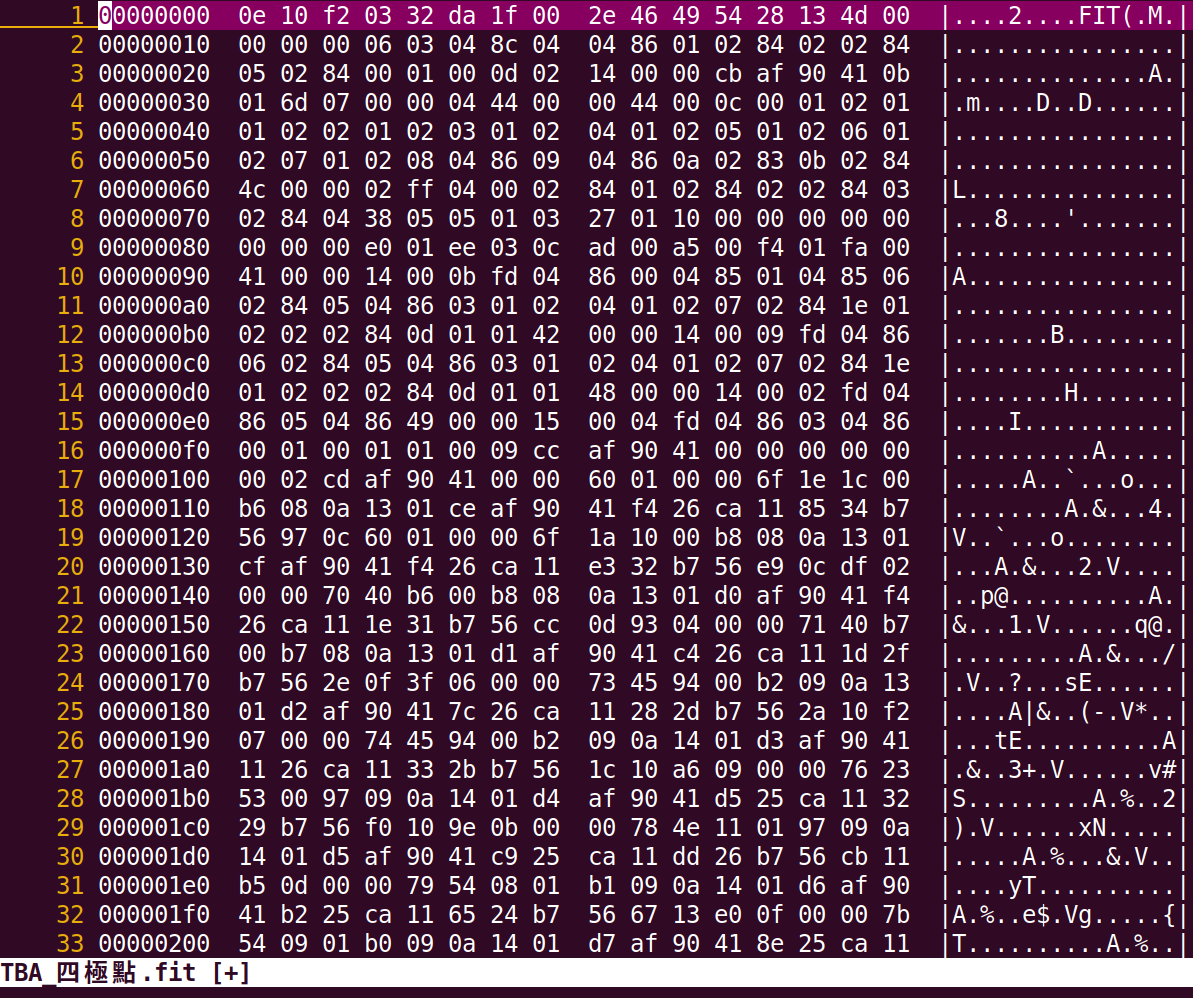
\includegraphics[width=7cm]{fit.png}
\end{multicols}
}
\end{itemize}
\end{frame}

\begin{frame}{編輯活動}
\only<1-3>{
\begin{itemize}
\item \href{https://github.com/brianhsu7476/activityEditPublish}{工具(持續更新中)}\pause
\item \href{https://www.facebook.com/profile.php?id=100009431154263}{工具人(持續忙碌中)}\pause
\item 還我河山騎錯路:\\
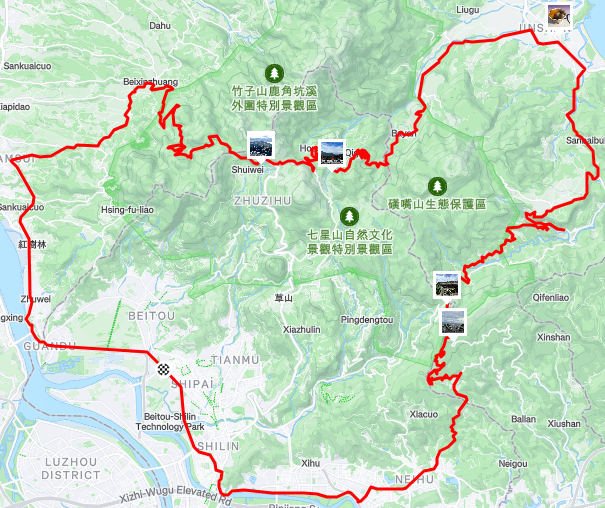
\includegraphics[width=7cm]{edit0.png}
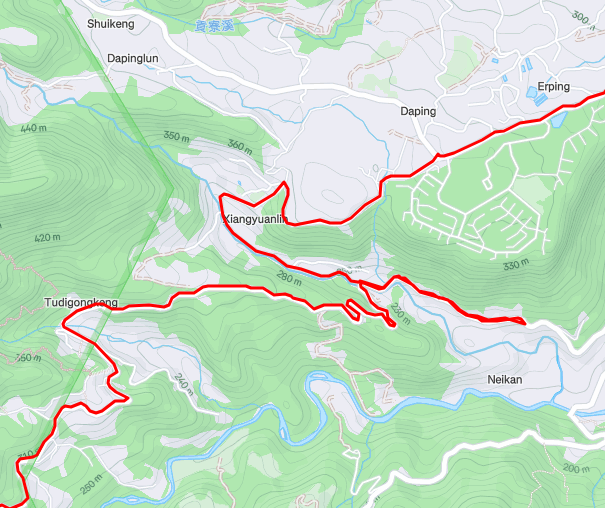
\includegraphics[width=7cm]{edit1.png}
\end{itemize}
}\only<4-5>{
\pause\pause\pause
\begin{itemize}
\item 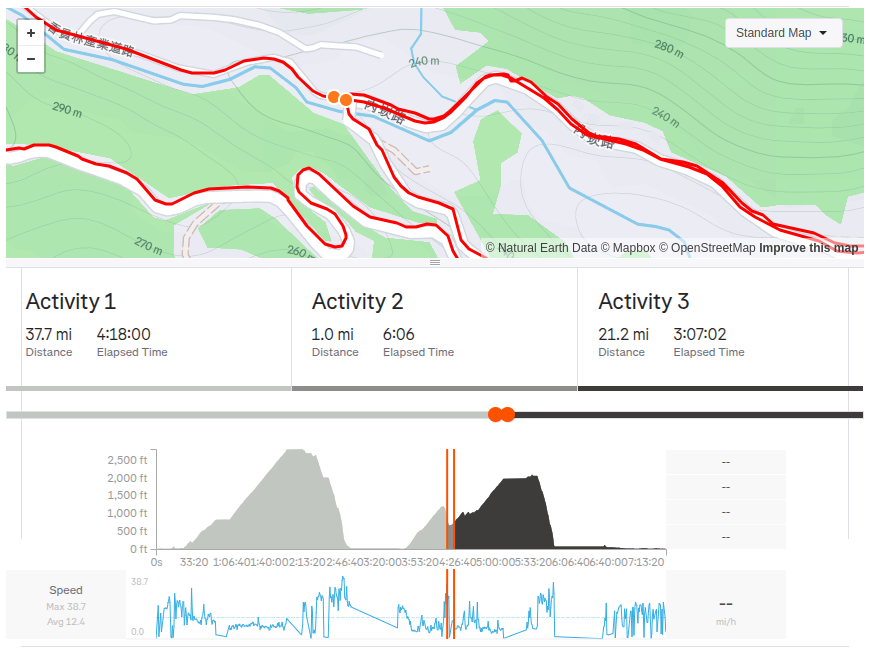
\includegraphics[width=7cm]{edit2.png}\pause
\item 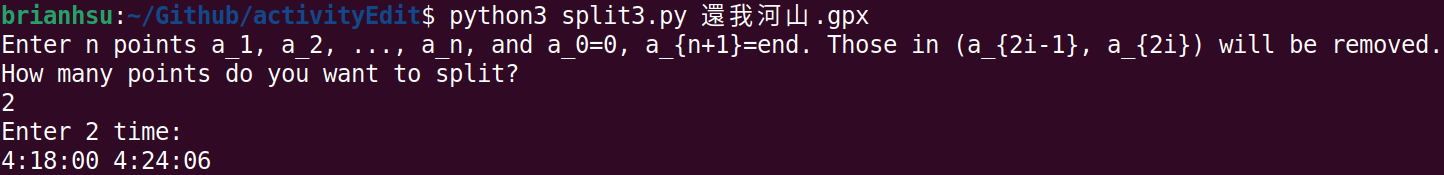
\includegraphics[width=14cm]{edit3.png}
\end{itemize}
}\only<6->{
\pause\pause\pause\pause\pause
\begin{multicols}{2}
\begin{itemize}
\item Before:\\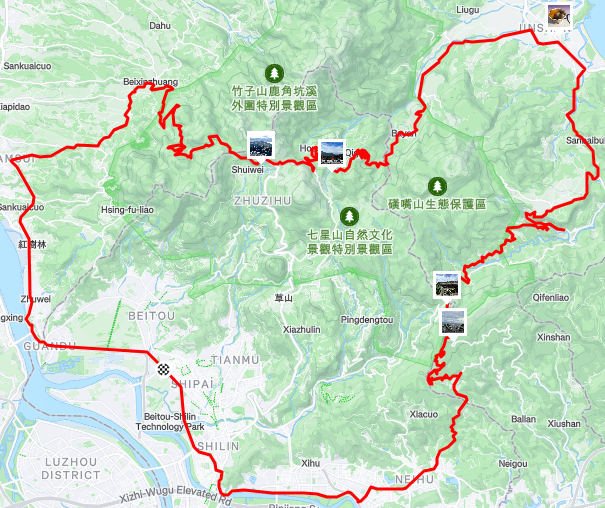
\includegraphics[width=7cm]{edit0.png}\pause
\item After:\\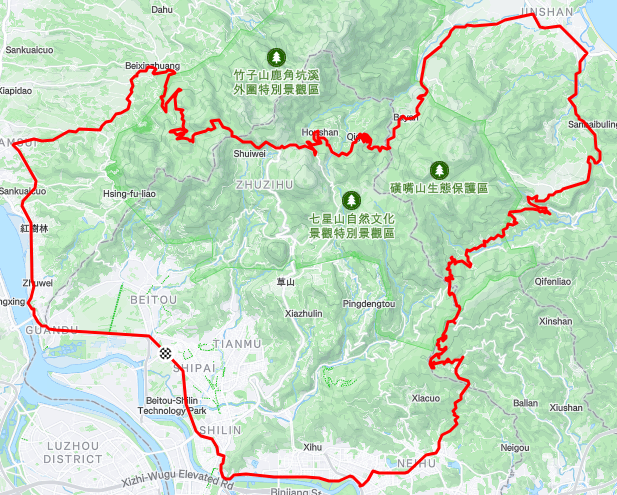
\includegraphics[width=7cm]{edit4.png}
\end{itemize}
\end{multicols}
}
\end{frame}

\begin{frame}{資訊讀書會}
\begin{itemize}
\item 繪製地圖的前後端處理\pause
\item 運動數據相關的 Machine Learning ,比如說給定一個人多個路段的成績,預測其騎武嶺的時間\pause
\item 爬蟲,把爬到的 .html 檔 parse 成能用的資料\pause
\item 資料蒐集,尋找關於運動員表現數據相關的 paper\pause
\end{itemize}
\begin{center}

\includegraphics[width=4cm]{IWantYou.jpeg}
\end{center}
\end{frame}
